\documentclass[11pt,final]{beamer}
\usepackage[czech]{babel}
\usepackage[T1]{fontenc}
\usepackage[utf8]{inputenc}
\usepackage{times}
\usepackage[linesnumbered, ruled, czech]{algorithm2e}
\usepackage{amsmath}
\usepackage{amsthm}
\usepackage{amsfonts}
\usepackage{hyperref}
\usepackage{tikz}


\title{Řadicí algoritmy}
\author{Domrachev Danil\\(xdomra00)}
\date{\today}

\setbeamertemplate{navigation symbols}{}	
\setbeamertemplate{footline}
{
	\begin{beamercolorbox}[right, sep=5ex]{}
		\insertframenumber/\inserttotalframenumber
	\end{beamercolorbox}
}
\usetheme{EastLansing}
\begin{document}
	%\mode<presentation>

	
	\begin{frame}
		\titlepage
	\end{frame}
	
	
	\begin{frame}[<+->]{Teorie}
		\begin{block}{}
			\structure{Algoritmus} -- konečná množina jednoduchých determinovaných kroků vedoucích k požadovanému cíli.
		\end{block}
		\vfill
		\onslide+<2->{Libovolný algoritmus lze zapsat pomocí tří komponent}
		\begin{itemize}

			\item[\phantom{x}] \phantom{text}\\
			\item<3->[$\bullet$] Sekvence\\
			\item<4->[$\bullet$] Selekce\\
			\item<5->[$\bullet$] Iterace	
		\end{itemize}
		\vfill
	\end{frame}


	\begin{frame}{Proč vůbec něco řadit?}
		Obvykle samotné řazení není konečným cílem, slouží k realizaci dalších algoritmů jako:
		\vfill
		\centering
		\onslide<2->{Algoritmy \alert{vyhledávání},}
	 	\onslide<3->{algoritmy \alert{datových struktur} atd.}
		\begin{figure}[h]
			\hspace{\stretch{0.1}}
			\pause
			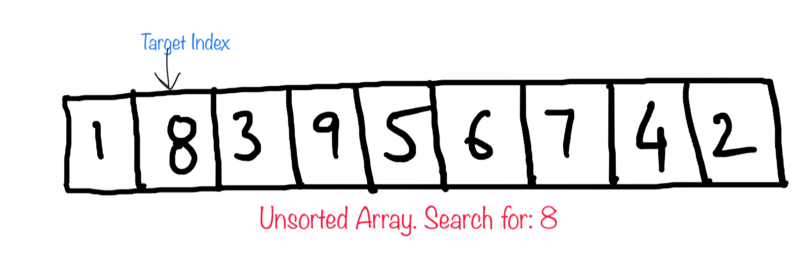
\includegraphics[scale=0.15,angle=35]{binsrc.png}
			\hspace{\stretch{0.3}}
			\pause
			\begin{tikzpicture}[scale=0.07]
				\tikzstyle{every node}+=[inner sep=0pt]
				\draw [black] (37.6,-8.2) circle (3);
				\draw [black] (39.6,-37.8) circle (3);
				\draw [black] (28.9,-22.3) circle (3);
				\draw [black] (55.8,-37.8) circle (3);
				\draw [black] (46.5,-22.3) circle (3);
				\draw [black] (34.1,-50.8) circle (3);
				\draw [black] (36.02,-10.75) -- (30.48,-19.75);
				\fill [black] (30.48,-19.75) -- (31.32,-19.33) -- (30.47,-18.8);
				\draw [black] (39.2,-10.74) -- (44.9,-19.76);
				\fill [black] (44.9,-19.76) -- (44.89,-18.82) -- (44.05,-19.35);
				\draw [black] (48.04,-24.87) -- (54.26,-35.23);
				\fill [black] (54.26,-35.23) -- (54.27,-34.28) -- (53.42,-34.8);
				\draw [black] (45.28,-25.04) -- (40.82,-35.06);
				\fill [black] (40.82,-35.06) -- (41.6,-34.53) -- (40.69,-34.13);
				\draw [black] (38.43,-40.56) -- (35.27,-48.04);
				\fill [black] (35.27,-48.04) -- (36.04,-47.5) -- (35.12,-47.11);
			\end{tikzpicture}	
		\hspace{\stretch{0.3}}
		\end{figure}
		\pause
		\raggedright
		Využitím seřazeného pole zvyšujeme jejich efektivitu
	\end{frame}

	\begin{frame}{Druhy řadicích algoritmů}
		\begin{figure}[h]
			\noindent
			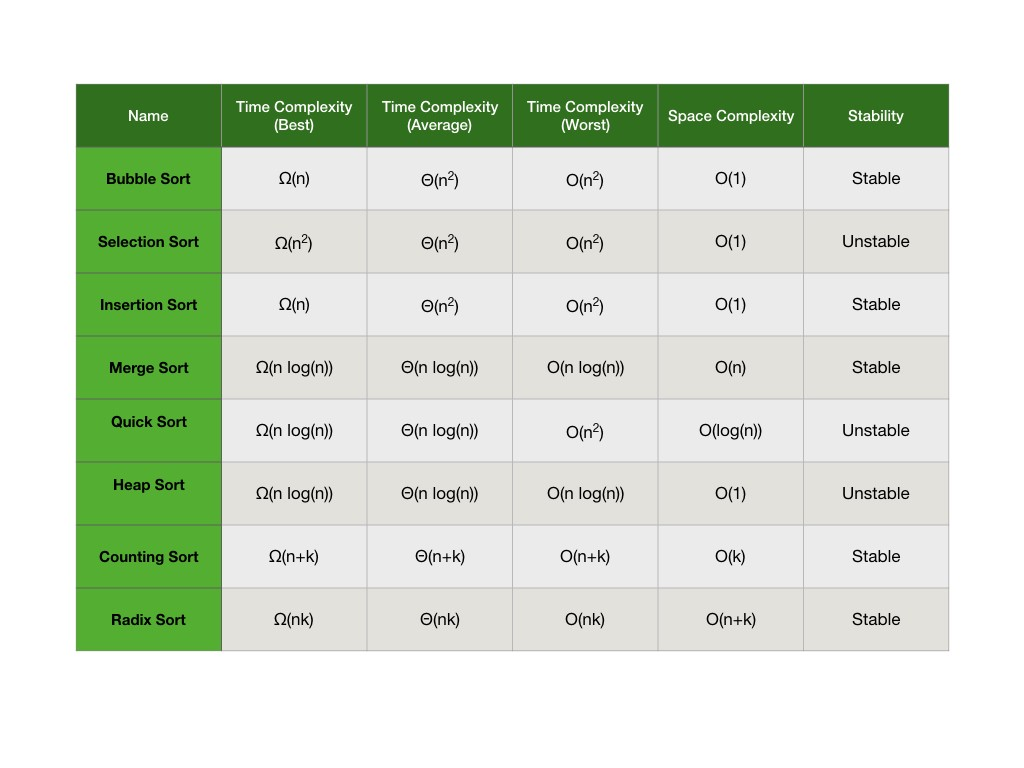
\includegraphics[scale=0.25]{algs.jpeg}
		\end{figure}
	\tiny \url{https://medium.com/@bill.shantang/8-classical-sorting-algorithms-d048eec3fdab}
	\end{frame}

	\begin{frame}{Vlastnosti řadicích algoritmů}
		\begin{itemize}
			\item<1->[$\bullet$]\structure{Stabilita} -- pořadí elementů se stejným klíčem se zachová\\
			\item<2->[$\bullet$]\structure{Způsob seřazení} -- obvykle porovnávím, ale existují i~jiné, \mbox{např. \alert{Counting Sort}}\\
			\item<3->[$\bullet$]\structure{Paralelita} -- dává možnost využít více procesorů současně pro zrychlení algoritmu\\
			\item<4->[$\bullet$]\structure{Přizpůsobivost} -- schopnost řadit rychleji na specificky předzpracovávaných datech\\
			\item<5->[$\bullet$]\structure{Prostorová náročnost} -- spotřeba paměti\\
			\item<6->[$\bullet$]\structure{Časová náročnost} -- rychlost seřazení 
		\end{itemize}
	\end{frame}

	\begin{frame}{Merge sort}
		\framesubtitle{Základní myšlenka: Rozděl a panuj}
		Drobíme pole až zůstanou skupiny ze dvou či jednoho prvku. Pak je postupně dáváme ve spravném pořadí do větších celků.
		\begin{figure}
			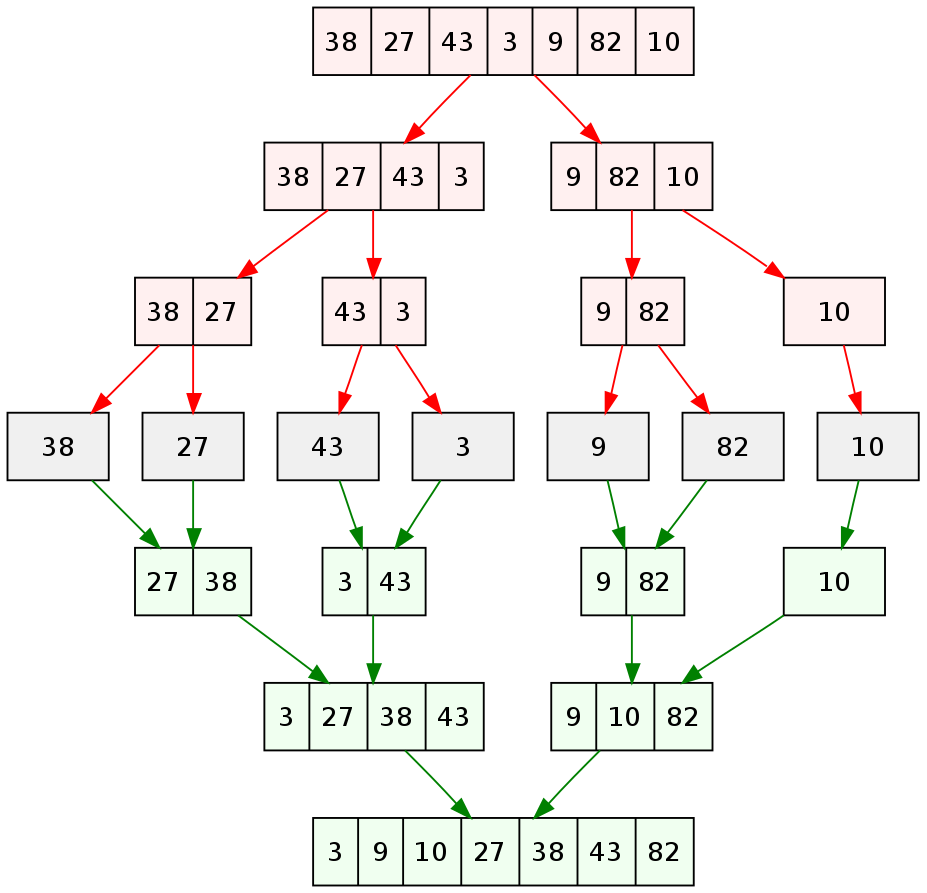
\includegraphics[scale=0.15]{wikimerge.png}
		\end{figure}
	\end{frame}

	\begin{frame}{Merge sort -- Realizace}
		\tiny
		\IncMargin{5em}
		\only<-1>{
		\begin{algorithm}[H]
			\DontPrintSemicolon
			\SetAlgoLongEnd
			\SetAlgoNoLine
			\SetNlSty{textmormal}{}{:}
			\SetKwInOut{Input}{Input}\SetKwInOut{Output}{Output}
			\Indm\Indm
			\caption{Help Function Merge()}
			\Indp\Indp
			
			\Input{$array, first, last$}
			\BlankLine
			$temp\_array = [\ ]$\;
			$middle = (first + last) / 2$\;
			$begin = first$\;
			$end = middle + 1$\;
			\For{$i = last$ \textbf{to} $end$}
			{
				\If{$(begin \leq middle)\;\&\;((end > last)\;\|\;(array[begin] < array[end]))$}
				{
					$temp\_array[i] = array[begin]$\;
					$begin = begin + 1$\;
				}
				\Else
				{
					$temp\_array[i] = array[end]$\;
					$end = end + 1$\;
				}
			}
			\For{$i = begin$ \textbf{to} $end$}
			{
				$array[i] = temp\_array[i]$\;
			}
			
		\end{algorithm}
		\DecMargin{5em}
		}
		\only<2->{
				\begin{algorithm}[H]
			\DontPrintSemicolon
			\SetAlgoLongEnd
			\SetAlgoNoLine
			\SetNlSty{textmormal}{}{:}
			\SetKwInOut{Input}{Input}\SetKwInOut{Output}{Output}
			\Indm\Indm
			\BlankLine
			\caption{Main Function MergeSort()}
			\Indp\Indp	
			\Input{$array, first, last$}
			\BlankLine
			\If{$first < last$}
			{
				$MergeSort(array, first, (first+last)/2)$\;
				$MergeSort(array, (first+last)/2 + 1, last)$\;
				$Merge(array, first, last)$\;
			}
			
		\end{algorithm}
	
		}	
	\end{frame}



\end{document}